\LARGE{ \textbf {Лекция №5}}\\

\Large{ \textbf { Минимизация логических функций с помощью карт Карно. }}\\
Получение минимальной дизъюнктивной нормальной формы
\begin{enumerate}
  \item Заполняются клетки карты Карно значениями функции
  \item Выделяются прямоугольные контуры, которые содержат в себе единички.
  Кол-во единиц в контуре должно быть равно $ N = 2^k \quad k \in 0 uN, \quad k = 1,2,3,4... \quad N = 1,2,4,8..$ клетка с единицей может принадлежать нескольким контурам. Контуры могут пересекаться. Кол-во контуров должно быть как можно меньше, но при условии, что все клетки с единицами охвачены. А размер контуров должен быть как можно больше. При выделении контуров считается, что верхняя строка и нижняя строка карты карно считаются соседними.
  Самый левый столбец и самый правый столбец так же считаются соседними.
  \item Записывается МДНФ. По следующим правилам: каждому контуру соответсвует терм, в который входят переменные, которые не меняют свое значение в пределах этого контура. В терме переменная берется без отрицания, если ее значение равно 1.
  И с отрицанием, если значение перменной равно 0  в пределах этого контура. Все получившиеся термы объединяются операцией дизъюнкции.
\end{enumerate}

Пример 1\\
$ y = \overline{a}bc + ab\overline{c} + abc \\
= \overline{a}bc + ab(\overline{c}+c)\\
= \overline{a}bc + ab\\
$
$
y = ab + bc
$


Получение минимальной конъюнктивной нормальной формы\\
В контуры объединяются клетки с нулями по тем же правилам.\\
В результате получает МДНФ для инверсного значения функции, а затем используя закон Де Могрга МДНФ преобразует в МКНФ.\\
$
\overline{f} = cd + \overline{a}b + b\overline{c} \\
f = \overline{cd} \cdot \overline{ \overline{a} b } \cdot \overline{b \overline{c}} \\
f = (\overline{c} + \overline{d}) \cdot (a + \overline{b}) \cdot (\overline{b} + c)
$

\Large{ \textbf { Неопределенные условия.}}\\
При синтезе логичсеких схем может возникнуть ситуация, что значение логической функции для некоторого входного набора не определенно,
либо данный входной набор запрещен.
В этом случае значение функции в карте карно помечают прочерком.
В картах карно такая клетка может включаться в единичные контуры, в нулевые, а может не включаться вообще.
Все зависит от нашей выгоды.\\
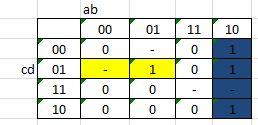
\includegraphics[width=\linewidth/2]{14}

$
f = a\overline{b} + \overline{a}b\overline{c}
$



\Large{ \textbf { Реализация логических функций в базисе И-НЕ, ИЛИ-НЕ}}\\
В схемотехнике базовыми элементами являются элементы И-НЕ, ИЛИ-НЕ.
Используя законы де Могргана можно получить представление аналитичесой функции удобное в реализации в базисе И-НЕ, ИЛИ-НЕ.\\
$
\overline{\overline{y}} = \overline{\overline{ab + bc}}
y = \overline{\overline{ab} \cdot \overline{bc}}
$

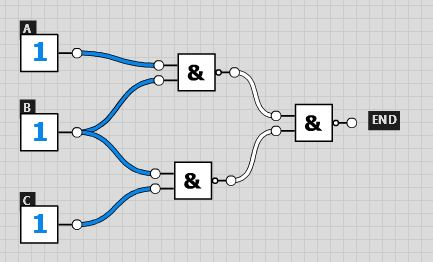
\includegraphics[width=\linewidth]{12}

Пример РК\\
Получить по заданной функции МДНФ и реализовать логическую схему.\\
$
y = \overline{a}\overline{b} + \overline{a}\overline{c} +\overline{b} \overline{d} + abcd
$

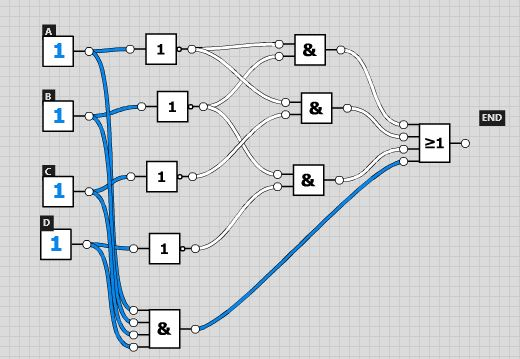
\includegraphics[width=\linewidth]{13}

Рекомендация: \\
Контуры овальные\\
У всех элементов входы слева, выходы справа.\\
Линии прямые. \\
\Large{ \textbf { Последовательсные схемы.
Триггерные схемы.}}

Структорной ячейкой в комбинационных схемах является логический элемент.\\
В основе последовательсных схем (схем с памятью) лежит триггер.\\
Триггер - устройство с 2 устойчивыми состояниями.\\
Пример электромеханического триггера является выключатель.\\

Обобщенная структурная схема триггера.\\
$x_1, x_n ;$ - информационные входы , $c_1, c_n$ - входы синхронизации\\
$Q$- прямой выход. $\overline{Q}$ - обратный выход.\\
Состяние триггера определяется его выходами.\\
Q = 0  $\overline{Q}$ = 1 триггер выключен.\\
Q = 1  $\overline{Q}$ = 0 триггер вкючен.\\
S` , R`  - сигналы, которые действуют на входы запоминающей ячейки.\\
S` - установка в 1.\\
R` - установка в 0.\\
Запоминающая ячейка - простейшая схема триггера.\\
